% docs/slides/preamble.tex -- 五份 deck 共享
\documentclass[aspectratio=169,11pt]{beamer}

% ==== 中文与字体 ====
\usepackage[UTF8,fontset=none]{ctex}
\usepackage{fontspec}

\IfFontExistsTF{PingFang SC}{%
  \setCJKmainfont{PingFang SC}[BoldFont=PingFang SC,ItalicFont=PingFang SC,AutoFakeSlant=0.15]
  \setCJKsansfont{PingFang SC}[ItalicFont=PingFang SC,AutoFakeSlant=0.15]
  \setCJKmonofont{PingFang SC}
}{%
  \IfFontExistsTF{Source Han Sans SC}{%
    \setCJKmainfont{Source Han Sans SC}
    \setCJKsansfont{Source Han Sans SC}
  }{%
    \IfFontExistsTF{Noto Sans CJK SC}{%
      \setCJKmainfont{Noto Sans CJK SC}
      \setCJKsansfont{Noto Sans CJK SC}
    }{%
      \setCJKmainfont{Heiti SC}
      \setCJKsansfont{Heiti SC}
    }
  }
}

\IfFontExistsTF{Helvetica Neue}{\setmainfont{Helvetica Neue}}{%
  \IfFontExistsTF{Inter}{\setmainfont{Inter}}{}}
\IfFontExistsTF{JetBrains Mono}{\setmonofont{JetBrains Mono}[Scale=0.85]}%
  {\setmonofont{Menlo}[Scale=0.85]}

% ==== 颜色 ====
\usepackage{xcolor}
\definecolor{cMain}{HTML}{1F4E79}
\definecolor{cAccent}{HTML}{E07A1F}
\definecolor{cGray}{HTML}{595959}
\definecolor{cMute}{HTML}{F4F4F4}
\definecolor{cOK}{HTML}{2E7D32}
\definecolor{cBad}{HTML}{B23A3A}
\definecolor{cWarn}{HTML}{C8A300}

% ==== 主题 ====
\usepackage{tcolorbox}
\usetheme{metropolis}
\metroset{progressbar=frametitle,numbering=fraction,block=fill}
\setbeamercolor{frametitle}{bg=cMain,fg=white}
\setbeamercolor{progress bar}{fg=cAccent,bg=cMute}
\setbeamercolor{alerted text}{fg=cAccent}
\setbeamercolor{title}{fg=cMain}

% metropolis 默认尝试 Fira Sans，未安装时 fallback 到 Latin Modern Sans。
% 这里在主题加载后显式覆盖，强制使用 macOS 上一定存在的 Helvetica Neue，
% 跟中文 PingFang 风格一致；找不到则按顺序尝试 Inter / Arial。
\IfFontExistsTF{Helvetica Neue}{%
  \setsansfont{Helvetica Neue}%
}{%
  \IfFontExistsTF{Inter}{\setsansfont{Inter}}{%
    \IfFontExistsTF{Arial}{\setsansfont{Arial}}{}}%
}

% ==== TikZ ====
\usepackage{tikz}
\usetikzlibrary{positioning,arrows.meta,fit,shapes.geometric,calc,%
  decorations.pathmorphing,backgrounds}

\tikzset{
  node-box/.style={draw=cMain,thick,rounded corners=2pt,
    minimum height=8mm,minimum width=18mm,align=center,font=\small},
  node-state/.style={draw=cMain,thick,circle,minimum size=14mm,
    align=center,font=\small},
  node-ok/.style={draw=cOK,thick,fill=cOK!10},
  node-warn/.style={draw=cWarn,thick,fill=cWarn!15},
  node-bad/.style={draw=cBad,thick,fill=cBad!10},
  % 色盲友好的状态机三态：蓝 (正常/Closed) / 橙 (告警/Open) / 灰 (中间/HalfOpen)
  % 避免 red-green 二元区分，改用 hue + lightness 双通道。
  node-state-normal/.style={draw=cMain,thick,fill=cMain!12},
  node-state-alert/.style={draw=cAccent,thick,fill=cAccent!18},
  node-state-transition/.style={draw=cGray,thick,fill=cGray!18},
  arrow/.style={-{Stealth[length=2mm]},thick,draw=cMain},
  arrow-async/.style={-{Stealth[length=2mm]},thick,dashed,draw=cGray},
  arrow-bad/.style={-{Stealth[length=2mm]},thick,draw=cBad},
  arrow-alert/.style={-{Stealth[length=2mm]},thick,draw=cAccent},
  lifeline/.style={dashed,thick,draw=cGray},
}

% ==== 代码 ====
\usepackage{listings}
\lstdefinelanguage{Go}{
  morekeywords={break,case,chan,const,continue,default,defer,else,
    fallthrough,for,func,go,goto,if,import,interface,map,package,range,
    return,select,struct,switch,type,var,nil,true,false,iota},
  morekeywords=[2]{string,int,int64,uint,uint64,bool,byte,error,context},
  sensitive=true,
  morecomment=[l]//,morecomment=[s]{/*}{*/},
  morestring=[b]",morestring=[b]`,
}
\lstdefinelanguage{LuaRedis}{
  morekeywords={and,break,do,else,elseif,end,false,for,function,if,in,
    local,nil,not,or,repeat,return,then,true,until,while},
  morekeywords=[2]{redis,call,KEYS,ARGV,tonumber,HGET,HSET,GET,SET,
    DECR,DECRBY,INCR,INCRBY,EXPIRE,PEXPIRE,ZADD,ZCARD,ZREMRANGEBYSCORE,
    EVAL,EVALSHA},
  sensitive=true,
  morecomment=[l]{--},
  morestring=[b]",morestring=[b]',
}

\lstdefinestyle{base}{
  basicstyle=\ttfamily\scriptsize,
  numbers=left,numberstyle=\tiny\color{cGray},
  keywordstyle=\color{cMain}\bfseries,
  keywordstyle=[2]\color{cAccent},
  stringstyle=\color{cOK},
  commentstyle=\color{cGray}\itshape,
  backgroundcolor=\color{cMute},
  frame=single,framerule=0pt,
  showstringspaces=false,
  breaklines=true,
  tabsize=2,
  columns=fullflexible,
}
\lstset{style=base}

% ==== 三线表与附录页码 ====
\usepackage{booktabs}
\usepackage{appendixnumberbeamer}

% ==== 页脚来源标注 ====
\newcommand{\srcnote}[1]{{\color{cGray}\scriptsize\itshape #1}}

% 关键论点框
\newcommand{\keypoint}[1]{%
  \begin{tcolorbox}[colback=cMute,colframe=cMain,boxrule=0.5pt,arc=2pt]%
  #1\end{tcolorbox}}


\title{营销活动}
\subtitle{优惠券 / 秒杀 / 抢红包 —— 业务取舍、ROI 与公平性}
\author{gomall · 业务侧 deck}
\date{}

\begin{document}

\maketitle

\begin{frame}{今日大纲}
\tableofcontents
\end{frame}

% ============================================================
\section{营销在 gomall 业务版图里的位置}
% ============================================================

\begin{frame}{为什么营销是一个独立 deck：业务视角的三条线}
\begin{itemize}
  \item gomall 主链路是\textbf{下单 → 支付 → 履约}，营销是\textbf{并行链路}：在用户开始下单决策\textbf{之前}动手。
  \item 三条业务线，目的截然不同：
  \begin{itemize}
    \item \textbf{优惠券}：促单 —— 把"看了不下单"的犹豫用户推过决策线。
    \item \textbf{秒杀}：引流 —— 用"亏本商品"换 UV / 新客 / APP 打开率。
    \item \textbf{抢红包}：留存 —— 让老用户每天有理由回来打开 APP。
  \end{itemize}
  \item 三条线共享一套底层武器：\textbf{Redis Lua 原子}、\textbf{滑动窗口反作弊}、\textbf{Saga 兜底}。
  \item 本 deck 关心两件事：(1) 每条线的业务取舍是什么 (2) 用同一套武器为什么能打三场不同的仗。
\end{itemize}
\srcnote{service/coupon.go, service/redpacket.go, service/skill\_goods.go 三个 service 入口}
\end{frame}

\begin{frame}{营销活动的 5 角色视图}
\scriptsize
\begin{tabular}{@{}lp{0.34\linewidth}p{0.42\linewidth}@{}}
\toprule
角色 & 营销活动对他意味着什么 & 他最怕看到什么 \\
\midrule
C 端用户   & "抢券、秒杀、抽红包"的兴奋时刻 & 抢券失败 / 红包金额很少 / 秒杀页面卡死 \\
商家       & 我的活动能引流多少？带来多少新客？ & 平台羊毛党把券都领走，真实用户没拿到 \\
运营       & 预算→GMV 的 ROI 算不算得过来 & 100 万发券，只换来 5 万 GMV 增量（ROI < 1） \\
客服       & 大促当天投诉量翻 5 倍，话术够不够用 & 用户问"为什么我抢不到红包"，没有标准回复 \\
SRE        & 流量峰值是平常 50×，集群扛得住吗 & 0 点限流误伤真用户 / Redis Lua 超时 \\
\bottomrule
\end{tabular}
\vspace{2mm}
\small \textbf{核心矛盾}：同一个活动，5 个角色的成功定义完全不同 ——\\
运营要"参与率高"，SRE 要"流量平稳"，客服要"话术清晰"，商家要"真客户拉到"，C 端用户要"抢得到 + 公平"。
本 deck 的每一帧都会回答："这个设计满足了谁，牺牲了谁。"
\srcnote{README 业务全景 5 角色表 + SLO P2 营销秒杀等级}
\end{frame}

\begin{frame}{业务承诺 SLO：营销是 P2，但峰值远超平日}
\begin{tabular}{@{}llll@{}}
\toprule
活动 & 业务等级 & 可用率 & p99 延迟 \\
\midrule
优惠券领取 & P2 营销 & 99\% & < 200ms \\
秒杀下单   & P2 营销 & 99\% & < 200ms \\
抢红包     & P2 营销 & 99\% & < 200ms（资金敏感建议 < 300ms） \\
\bottomrule
\end{tabular}
\vspace{2mm}
\small \textbf{P2 不是次要}：用户的购物决策\textbf{在大促当天集中爆发}，营销失败意味着"用户走了，整年的 GMV 都拉不回"。\\
\textbf{流量画像}：平日营销接口 100 QPS，大促 0 点 5--10 万 QPS（50--100×）。
\vspace{2mm}
\begin{itemize}
  \item \textbf{宁可下游慢、不能上游 429}：营销可以排队、可以"已抢完"，但\textbf{不能 5xx 让用户看到崩溃}。
  \item \textbf{99\% 可用率的潜台词}：可以接受全场 1\% 用户被限流误伤，但不接受 1\% 用户超发（资损）。
  \item \textbf{P2 的代价}：实测压测 30VU × 15s 通过 46 / 期望 45 / \textbf{误差 2.2\%} —— 误伤 < 5\% 才算合格。
\end{itemize}
\srcnote{README SLO 表 P2 营销秒杀；stressTest/REPORT.md \S 5 限流压测}
\end{frame}

\begin{frame}{业务边界：这份 deck 覆盖什么、不覆盖什么}
\begin{tikzpicture}[node distance=4mm and 6mm]
  \node[node-box,node-ok]   (in1) {优惠券领取};
  \node[node-box,node-ok,right=of in1] (in2) {秒杀抢购};
  \node[node-box,node-ok,right=of in2] (in3) {抢红包};
  \node[node-box,below=of in1,node-bad] (out1) {AB 测试};
  \node[node-box,right=of out1,node-bad] (out2) {用户分群};
  \node[node-box,right=of out2,node-bad] (out3) {满减引擎};
  \node[node-box,below=of out1,node-bad] (out4) {会员等级};
  \node[node-box,right=of out4,node-bad] (out5) {积分体系};
  \node[node-box,right=of out5,node-bad] (out6) {拼团 / 直播};
\end{tikzpicture}
\vspace{2mm}
\small \textbf{做了的}（绿）：三个核心 Lua 原子机制 + Saga 兜底 + 限流防黑产 + 客服话术映射。\\
\textbf{没做的}（红）：\textbf{AB 测试} / \textbf{用户分群} / \textbf{满减折扣引擎} / \textbf{商家自助活动配置} / \textbf{积分} / \textbf{会员等级} / \textbf{拼团} / \textbf{直播带货}。\\
\textbf{为什么不做}：这些是\textbf{运营 / 商家工作台}的事，gomall 当前阶段聚焦"\textbf{交易闭环 + 防资损}"。等 wallet 与 merchant 服务落地后再做。
\srcnote{README "业务边界（不做什么）" 段；docs/architecture/feature-matrix.md}
\end{frame}

% ============================================================
\section{优惠券：促单工具 + ROI 计算}
% ============================================================

\begin{frame}{优惠券的业务目的：把犹豫用户推过决策线}
\begin{itemize}
  \item \textbf{业务公式}：商品定价 100 元，用户犹豫 → 发 20 元券 → 净付 80 元 → 下单。\\
        平台损失 20 元，但换来\textbf{一笔本来不会发生的订单}（GMV +80）。
  \item \textbf{触达分层}：
  \begin{itemize}
    \item \textbf{新客券}：注册赠送 50 元，目的是\textbf{首单转化}（行业 LTV 计算依赖首单完成）。
    \item \textbf{老客回流券}：90 天未下单触发，目的\textbf{召回沉睡用户}。
    \item \textbf{大促预热券}：提前 7 天发，让用户"提前决策"，0 点不挤兑结算系统。
  \end{itemize}
  \item \textbf{为什么必须"先领后用"}：让用户产生"沉没成本错觉" —— 已经领了的券\textbf{不用就亏了}。
  \item \textbf{gomall 现状}：只做最基础的"批次 + 单人限领"，没做触达分层（运营平台路线图）。
\end{itemize}
\srcnote{model.CouponBatch.Type/Threshold/Amount 字段；service/coupon.go:30--57 CreateBatch}
\end{frame}

\begin{frame}{活动 ROI 业务化帧：100 万发券能换多少 GMV}
\scriptsize \textbf{运营视角}：一次活动是不是值，看这张表。
\begin{tabular}{@{}lrrr@{}}
\toprule
环节 & 行业基准 & 算式 & 数值 \\
\midrule
发券量            & 50000 张 (满 100 减 20)  & 单券面值 20 元 & 预算 \textbf{100 万} \\
领取率            & 60\% (券进了用户卡包)    & 50000 × 60\% & 30000 张已领 \\
核销率            & 20\% (实际下单使用)      & 30000 × 20\% & 6000 张已用 \\
带动 GMV          & 用券单平均客单 150 元    & 6000 × 150 & \textbf{90 万} \\
平台让利          & 实际抵扣金额             & 6000 × 20 & \textbf{12 万} \\
拉新效应          & 新客占用券 30\%          & 6000 × 30\% & 1800 新客 \\
\midrule
\textbf{ROI 计算} & GMV / 让利               & 90 万 / 12 万 & \textbf{7.5} \\
\bottomrule
\end{tabular}
\vspace{2mm}
\small \textbf{运营怎么判合格}：核销率 20\% \& ROI > 5 算合格。低于 10\% 核销率 = 券面值太低/门槛太高，用户懒得用。\\
\textbf{被黑产吃掉的代价}：如果 30\% 券进了脚本党的手里（领了不用 / 倒卖），\textbf{真实拉新打 7 折，核销率打 7 折，整个 ROI 直接腰斩}。这就是下文限流的钱字号意义。
\srcnote{README 业务承诺 + service/coupon.go Claim 流程；ROI 算式为行业常识、gomall 未实装}
\end{frame}

\begin{frame}{coupon 接口的中间件链：业务诉求决定每一层}
\begin{tikzpicture}[node distance=4mm and 7mm]
  \node[node-box] (cli) {Client};
  \node[node-box,right=of cli,node-warn] (gw) {TokenBucket\\100/IP};
  \node[node-box,right=of gw] (auth) {JWT};
  \node[node-box,right=of auth,node-ok] (lua) {coupon Lua\\原子扣减};
  \node[node-box,below=of lua] (tx) {DB Tx\\PersistClaim};
  \node[node-box,left=of tx,node-bad] (rb) {Rollback Lua\\Incr+Decr};
  \draw[arrow] (cli) -- (gw); \draw[arrow] (gw) -- (auth);
  \draw[arrow] (auth) -- (lua); \draw[arrow] (lua) -- (tx);
  \draw[arrow-bad,bend right=20] (tx.west) to node[above,font=\tiny]{DB FAIL} (rb.east);
\end{tikzpicture}
\vspace{2mm}
\small \textbf{业务取舍}：coupon 链路\textbf{故意做轻}，只挂全局 TokenBucket。原因——
\begin{itemize}\itemsep0pt
  \item 业务侧\textbf{鼓励多领}：用户每多领一张就多一份"沉没成本"，转化率正相关。
  \item Lua 里已经管控了 \textbf{PerUser 单人上限}，业务码 \texttt{-2} 直接挡。
  \item 单独挂 SlidingWindow 反而限制活跃用户（频繁刷新页面也会被截）。
\end{itemize}
\textbf{代价}：万号脚本党可以慢慢扫。靠 IP TokenBucket + 风控（路线图）兜底。
\srcnote{routes/router.go:22 全局桶；:70--73 coupon 路由（无 SlidingWindow）}
\end{frame}

\begin{frame}[fragile]{coupon Lua：库存 + 单人限领 二维原子}
\small \textbf{业务约束}：两道闸\textbf{必须同时锁}—— 先 DECR 再判单人 = 已超限请求会留"幽灵库存"。代码顺序是有讲究的。
\begin{lstlisting}[language=LuaRedis,firstnumber=30,
  caption={\srcnote{repository/cache/coupon.go:30--44 claimScript}}]
local stock = tonumber(redis.call('GET', KEYS[1]))
if stock == nil or stock <= 0 then
    return -1                                  -- 已抢光
end
local owned = tonumber(redis.call('GET', KEYS[2]))
if owned == nil then owned = 0 end
if owned >= tonumber(ARGV[1]) then
    return -2                                  -- 超出单人上限
end
redis.call('DECR', KEYS[1])
redis.call('INCR', KEYS[2])
redis.call('EXPIRE', KEYS[2], tonumber(ARGV[2]))
return 1
\end{lstlisting}
\vspace{-1mm}
\scriptsize \textbf{业务码映射}：\texttt{1 → 200 成功}；\texttt{-1 → "已抢光" 终态}；\texttt{-2 → "每人限领 N 张"}。Lua 返回 \texttt{int}，Go 侧 switch 翻译成 \texttt{ErrCouponSoldOut / ErrCouponPerUserExceed}（无独立业务码，复用 ERROR=500 + 文案）。
\srcnote{repository/cache/coupon.go:57--75 ClaimCouponAtomic 翻译错误码}
\end{frame}

\begin{frame}{coupon 压测数字：业务侧怎么解读这两组数据}
\begin{minipage}[t]{0.46\linewidth}
\scriptsize
\begin{tabular}{@{}lrr@{}}
\toprule
& Redis Lua & DB FOR UPDATE \\
\midrule
500 并发抢 100 张 & 零超发 & 零超发 \\
吞吐 RPS          & 51{,}362 & 50{,}142 \\
avg 延迟          & 0.82ms   & 0.83ms  \\
\textbf{max 延迟} & \textbf{136ms} & \textbf{453ms} \\
\bottomrule
\end{tabular}
\end{minipage}
\hfill
\begin{minipage}[t]{0.50\linewidth}
\scriptsize \textbf{业务侧解读}：吞吐拉平不等于体验一样。\\
- \textbf{尾延迟差 3.3×}：DB 锁路径下，500 个用户里有几个会等 0.45s。\\
- 用户感知：DB 路径 = "刷新两次才出结果"。\\
- 大促日叠加重试 = 雪崩。\\
\textbf{结论}：吞吐看 avg，体验看 p99 / max。
\end{minipage}
\vspace{2mm}

\small \textbf{零超发是底线}：1000 goroutine 抢 100 张券 → 成功数恰好 100，DB 行数 100，Redis 库存归 0，三者一致。\\
\textbf{业务侧再次确认}：这个不是技术指标，这是"\textbf{不被资损}"的底线 —— 多发出去一张券就是真金白银的损失。
\srcnote{stressTest/REPORT.md 链路压测表 第 5--6 行；repository/cache/coupon.go:30--44}
\end{frame}

% ============================================================
\section{秒杀：亏本引流 + 流量峰值}
% ============================================================

\begin{frame}{秒杀的业务本质：用"亏本商品"换"全场曝光"}
\begin{itemize}
  \item \textbf{业务公式}：iPhone 标价 8000 元，秒杀价 999 元 → 100 台 → 平台亏\textbf{70 万}。\\
        但带来\textbf{全场 500 万 UV} + \textbf{APP 当日打开率 +30\%} + \textbf{大量"陪跑"用户顺手买别的}。
  \item \textbf{ROI 拆解}：
  \begin{itemize}\itemsep0pt
    \item 直接亏损：70 万（秒杀差价）
    \item 间接 GMV：500 万 UV × 0.5\% 陪跑转化 × 客单 200 = \textbf{500 万}
    \item 新增日活：APP 当日 DAU +30\%（次日留存 30--40\%，长期 LTV 收益）
  \end{itemize}
  \item \textbf{业务取舍}：\textbf{秒杀必须有"抢不到"的人}。如果 100 台 iPhone 5 分钟才卖完，那不叫秒杀。\textbf{用户预期是"瞬间售罄"}，没抢到不是产品问题，是\textbf{运气问题}。
  \item \textbf{对应客服话术}：从来不说"系统繁忙"，永远说"\textbf{已被其他用户抢走，欢迎下次参与}"。
\end{itemize}
\srcnote{service/skill\_goods.go:122--134 SkillProduct；商品独立 model.SkillProduct 表}
\end{frame}

\begin{frame}{秒杀 vs 普通下单的根本差异：业务侧规则}
\scriptsize
\begin{tabular}{@{}lp{0.32\linewidth}p{0.44\linewidth}@{}}
\toprule
维度 & 普通下单 & 秒杀 \\
\midrule
\textbf{商品池}      & Product 主表 & 独立 \texttt{SkillProduct} 表 \\
\textbf{库存}        & 与展示页同步 & 单独预热到 Redis，与主商品池隔离 \\
\textbf{用户预期}    & 总能下单 & 大概率抢不到 \\
\textbf{重复点击}    & 业务上是 bug & 业务上是\textbf{常态}（用户疯狂点击） \\
\textbf{失败的语义}  & "服务挂了" & "你手慢了" \\
\textbf{限流策略}    & 不挂限流（P0） & 强制 SlidingWindow 3/s/用户 \\
\textbf{熔断策略}    & 可熔断到熔断器返回降级 & \textbf{不熔断} \\
\bottomrule
\end{tabular}
\vspace{2mm}

\small \textbf{为什么秒杀不熔断}：熔断 = "所有人都买不到"，业务上等价于\textbf{活动作废} —— 比"部分用户买不到"严重 10 倍。\\
\textbf{为什么秒杀不挂 Idempotency}：用户疯狂点击"再试一次"\textbf{就是业务预期}，幂等命中会让用户以为下单成功，反而误导。
\srcnote{service/skill\_goods.go:122--134；routes/router.go:142--152 秒杀路由}
\end{frame}

\begin{frame}{SlidingWindow Lua 与"阈值 = 3"的业务依据}
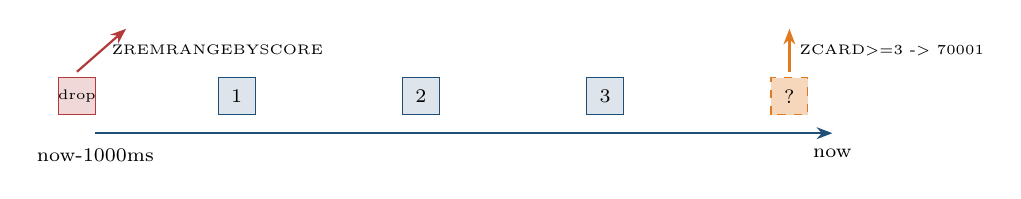
\begin{tikzpicture}[scale=0.78, every node/.style={font=\scriptsize}]
  \draw[arrow] (0,0) -- (12,0);
  \node[below] at (0,-0.1) {now-1000ms};
  \node[below] at (12,-0.1) {now};
  % 旧请求
  \draw[fill=cBad!20,draw=cBad] (-0.6,0.3) rectangle (0.0,0.9);
  \node[font=\tiny] at (-0.3,0.6) {drop};
  \draw[arrow-bad] (-0.3,1.0) -- node[right,font=\tiny]{ZREMRANGEBYSCORE} (0.5,1.7);
  % 窗口内
  \draw[fill=cMain!15,draw=cMain] (2,0.3) rectangle (2.6,0.9);
  \draw[fill=cMain!15,draw=cMain] (5,0.3) rectangle (5.6,0.9);
  \draw[fill=cMain!15,draw=cMain] (8,0.3) rectangle (8.6,0.9);
  \node at (2.3,0.6) {1};
  \node at (5.3,0.6) {2};
  \node at (8.3,0.6) {3};
  % 待入
  \draw[fill=cAccent!30,draw=cAccent,dashed] (11.0,0.3) rectangle (11.6,0.9);
  \node at (11.3,0.6) {?};
  \draw[arrow-alert] (11.3,1.0) -- node[right,font=\tiny]{ZCARD>=3 -> 70001} (11.3,1.7);
\end{tikzpicture}
\vspace{2mm}
\small \textbf{业务侧选阈值的依据}：
\begin{itemize}\itemsep0pt
  \item 真人最快\textbf{300--500ms 点一次}，1 秒内 2--3 次封顶（除非用脚本）。
  \item 阈值 = 3 留 50\% 余量给\textbf{网络抖动 / 手抖连点 / 主动重试}。
  \item 阈值 = 10 形同没限（一台脚本 1 秒打 50 次都过）。
  \item 阈值 = 1 \textbf{客诉爆炸}（用户网络稍差就被截）。
\end{itemize}
\textbf{业务码 70001}：限流命中，客服话术"\texttt{操作过于频繁，请稍后再试}"，\textbf{不是失败、不是错误}，是"\texttt{稍等 1 秒重试就行}"。
\srcnote{repository/cache/ratelimit.go:18--34 SlidingWindow Lua；pkg/e/code.go:57 ErrRateLimitExceeded=70001}
\end{frame}

\begin{frame}{秒杀压测实测：30VU × 15s 误差 2.2\%}
\textbf{场景}：30 个并发用户用\textbf{同一 token}打 \texttt{/skill\_product/skill}，配置 \texttt{Limit=3 Window=1s ByUser=true}（模拟"\textbf{一个账号被脚本疯狂调用}"的黑产画像）。

\vspace{2mm}
\begin{tabular}{@{}lrr@{}}
\toprule
指标 & 实测 & 业务期望 \\
\midrule
通过请求数 & 46  & 15s × 3 = 45 \\
被限流数   & 781{,}624 & 黑产应全部拦下 \\
误差       & 2.2\% & < 5\% 合格 \\
\bottomrule
\end{tabular}
\vspace{3mm}

\small \textbf{业务侧解读}：
\begin{itemize}\itemsep0pt
  \item "通过 46 次" $\approx$ 真用户最快也只能秒到 45 次/15s，业务合理。
  \item 被截 \textbf{78 万次都是同一 token} = 标准黑产画像。
  \item 误差 2.2\% 对运营说"\textbf{合规}"，对 SRE 说"\textbf{压力可控}"，对客服说"\textbf{真用户极少误伤}"。
\end{itemize}
\textbf{大促 SOP 联动}：监控大盘看\textbf{被限流数 / 通过数比值}，如果飙升 = 黑产攻击，运营触发风控降级。
\srcnote{stressTest/REPORT.md \S 5 限流中间件压测；seckill\_rate\_limit.js 脚本}
\end{frame}

\begin{frame}{秒杀客诉链路：从"我抢不到"到客服话术}
\begin{tikzpicture}[node distance=5mm and 10mm]
  \node[node-box] (u) {用户};
  \node[node-box,right=of u] (api) {API};
  \node[node-box,right=of api,node-warn] (sw) {SlidingWindow};
  \node[node-box,right=of sw,node-ok] (lua) {库存\\Lua};
  \node[node-box,below=of api,node-warn] (cs1) {话术 A\\70001 限流};
  \node[node-box,below=of sw,node-warn]  (cs2) {话术 B\\已抢光};
  \node[node-box,below=of lua,node-warn] (cs3) {话术 C\\已领过};
  \draw[arrow-bad] (sw) -- node[right,font=\tiny]{70001} (cs1.east);
  \draw[arrow-bad] (lua.south) -- node[right,font=\tiny]{stock=0} (cs2.north);
  \draw[arrow-bad] (lua) -- node[right,font=\tiny]{owned>=N} (cs3.north);
\end{tikzpicture}
\vspace{2mm}
\small \textbf{客服必须区分三种"失败"}：
\begin{itemize}\itemsep0pt
  \item \textbf{70001 限流}："操作过于频繁，请稍后再试"——\textbf{1 秒后可重试}。
  \item \textbf{库存 = 0 已抢光}："已被其他用户抢走，欢迎下次参与"——\textbf{终态、不可重试}。
  \item \textbf{owned $\geq$ N 已领过}："您已成功参与本次活动"——\textbf{鼓励、不打击用户}。
\end{itemize}
\textbf{用户体验红线}：\textbf{绝不能}说"系统繁忙"或"未知错误" —— 用户会以为是 bug，立刻投诉。
\srcnote{pkg/e/code.go:57--58 70001/70002；repository/cache/coupon.go 错误码翻译}
\end{frame}

% ============================================================
\section{抢红包：公平性是用户体验生死线}
% ============================================================

\begin{frame}{抢红包的业务目的：留存而非促单}
\begin{itemize}
  \item \textbf{业务公式}：发 1000 个 1 元红包 → 1000 人参与 → 抢到的"开心"+ 没抢到的"下次还来"。\textbf{钱花得不多，留存效果惊人}。
  \item \textbf{核心差异}：和优惠券（促单）、秒杀（引流）不同 —— 红包\textbf{不直接 GMV 转化}，目的是\textbf{每日打开率 / 7 日留存率}。
  \item \textbf{发包场景}：商家发（送老客）、平台发（节日大礼）、用户互发（社交裂变 —— gomall 当前是个人钱包发）。
  \item \textbf{业务关键点 1：金额必须随机}。如果每人 1 元 = 优惠券，不刺激；要有人抢到 5 元，有人抢到 1 分。
  \item \textbf{业务关键点 2：总额必须精确}。100 元发出去就是 100 元，多 1 分平台亏、少 1 分用户投诉。
  \item \textbf{业务关键点 3：公平感}。\textbf{每份 ≥ 1 分} + 顺序打散 + 最后一份兜底 —— 这是用户口碑的生死线。
\end{itemize}
\srcnote{service/redpacket.go:42--103 Create + Claim 全流程}
\end{frame}

\begin{frame}{公平性事故的真实代价：业务案例}
\textbf{反面教材}：某红包活动 \textbf{1000 元 / 100 份} 拆分时 bug 让\textbf{第 1 个抢到的人独占 800 元}，剩下 99 人抢 200 元（平均 2 元）。

\vspace{1mm}
\begin{tabular}{@{}lp{0.72\linewidth}@{}}
\toprule
现象 & 后果 \\
\midrule
社交媒体爆款 & 截图被疯传"\textbf{XX 公司抢红包内定}"，活动 ROI 直接归零 \\
品牌信任崩塌 & 用户下次活动\textbf{不参与}：反正抢不到大头 \\
监管关注     & 涉嫌\textbf{诱导分享 + 不公平算法}，运营部约谈 \\
内部追责     & 算法工程师 + 产品 + QA 三方追责（这种 bug \textbf{压测覆盖不到}） \\
真实修复成本 & 给\textbf{所有参与者补发}红包 + 公开道歉 + 算法外审 \\
\bottomrule
\end{tabular}
\vspace{2mm}

\small \textbf{业务结论}：抢红包的"公平感" $\neq$ "金额平均" —— 用户能接受抢到 1 分，但\textbf{不能接受规则可疑}。\\
gomall 用\textbf{二倍均值法}保证：(1) 每份 $\geq$ 1 分 (2) 总额守恒 (3) Shuffle 打散位置敏感。三件事任一缺失就是上述事故。
\srcnote{repository/cache/redpacket.go:98--142 SplitRedPacket}
\end{frame}

\begin{frame}[fragile]{二倍均值法：业务约束如何映射成代码}
\small \textbf{业务约束 → 算法选择}：
\begin{itemize}\itemsep0pt
  \item "总额精确" → 最后一份 \texttt{out[count-1] = remain} \textbf{兜底吃剩}。
  \item "每份 $\geq$ 1 分" → 随机区间 \texttt{[1, hi]}，\texttt{maxThisRound = remain - (剩余份数)} 保证后续每份至少 1。
  \item "随机有惊喜" → 上界 \texttt{2*avg-1}，期望 = avg，方差由 avg 控制。
  \item "位置不敏感" → 最后 \texttt{Shuffle} 打散数组，否则用户能推断"第一个抢的最大"。
\end{itemize}
\begin{lstlisting}[language=Go,firstnumber=98,
  caption={\srcnote{repository/cache/redpacket.go:98--142 SplitRedPacket}}]
out := make([]int64, count)
remain := total
for i := 0; i < count-1; i++ {
    left := int64(count - i)
    avg := remain / left * 2                  // [1, 2*avg-1] 区间上界
    if avg < 2 { avg = 2 }
    maxThisRound := remain - int64(count-1-i) // 留 1 分给后面每份
    hi := avg - 1
    if hi > maxThisRound { hi = maxThisRound }
    if hi < 1 { hi = 1 }
    amt := splitRand.r.Int63n(hi) + 1         // [1, hi] 闭区间
    out[i] = amt; remain -= amt
}
out[count-1] = remain                          // 最后一份兜底
splitRand.r.Shuffle(count, ...)                // 打散
\end{lstlisting}
\end{frame}

\begin{frame}{200 元 / 10 份分布示意 + 用户感知}
\begin{tikzpicture}[scale=0.8, every node/.style={font=\scriptsize}]
  \draw[arrow] (0,0) -- (11,0);
  \node[below] at (0,0)  {第 1 份};
  \node[below] at (5.5,0){第 5 份};
  \node[below] at (10,0) {第 10 份};
  \draw[fill=cMain!30] (0,0) rectangle (1,2.3);
  \draw[fill=cMain!30] (1,0) rectangle (2,1.8);
  \draw[fill=cMain!30] (2,0) rectangle (3,2.1);
  \draw[fill=cMain!30] (3,0) rectangle (4,1.6);
  \draw[fill=cMain!30] (4,0) rectangle (5,2.0);
  \draw[fill=cMain!30] (5,0) rectangle (6,1.9);
  \draw[fill=cMain!30] (6,0) rectangle (7,2.2);
  \draw[fill=cMain!30] (7,0) rectangle (8,1.7);
  \draw[fill=cMain!30] (8,0) rectangle (9,2.5);
  \draw[fill=cAccent!50] (9,0) rectangle (10,1.9);
  \draw[dashed,cGray] (0,2.0) -- (10,2.0) node[right,font=\tiny] {avg=20};
\end{tikzpicture}
\vspace{2mm}

\small \textbf{用户视角}：抢到 25 元的觉得"\textbf{运气真好}"，抢到 16 元的觉得"\textbf{还行}"，抢到 0.01 元的会发朋友圈"\textbf{手慢了哈哈}"。\\
\textbf{产品价值}：每份不等 → 每个人都\textbf{有故事讲} → 社交传播 → 下次活动\textbf{自发参与}。\\
\textbf{对比反面}：等额拆分 = 100 元 / 100 份 = 每人 1 元 → 没人晒图 → 留存效果归零。
\srcnote{repository/cache/redpacket.go:113--141；行业经验：拼手气红包 vs 等额红包的留存对比}
\end{frame}

\begin{frame}[fragile]{抢红包 Lua：业务规则 8 行落地}
\small \textbf{业务规则三句话}：(1) \textbf{一个人只能抢一次} (2) \textbf{抢完即终止} (3) \textbf{抢到金额是哪一份就是哪一份}。
\begin{lstlisting}[language=LuaRedis,firstnumber=52,
  caption={\srcnote{repository/cache/redpacket.go:52--63 claimRedPacketScript}}]
if redis.call('HEXISTS', KEYS[2], ARGV[1]) == 1 then
    return -2                                 -- 已领过
end
local amt = redis.call('LPOP', KEYS[1])
if not amt then
    return -1                                 -- 已抢完
end
redis.call('HSET', KEYS[2], ARGV[1], amt)
redis.call('EXPIRE', KEYS[2], tonumber(ARGV[2]))
return tonumber(amt)                          -- 抢到金额
\end{lstlisting}
\vspace{-1mm}
\scriptsize \textbf{业务码翻译}（Go 侧 \texttt{repository/cache/redpacket.go:165--189}）：\\
\texttt{-1 → ErrRedPacketDrained} → 客服话术 "\texttt{红包已被抢完}"（README 称作 \texttt{RP-EMPTY} 文案，代码侧是 Go error）\\
\texttt{-2 → ErrRedPacketAlreadyTaken} → 客服话术 "\texttt{您已领取过本红包}"\\
\texttt{> 0 → 200 + amount} → 客户端展示动画
\end{frame}

\begin{frame}{抢红包 Saga：资金链路的"最后一道防线"}
\begin{tikzpicture}[node distance=7mm and 12mm]
  \node[node-box,node-ok] (lua) {Lua\\LPOP 50 分};
  \node[node-box,right=of lua] (db) {DB Tx\\写 claim + outbox};
  \node[node-box,right=of db,node-bad] (fail) {Tx Fail};
  \node[node-box,below=of fail,node-warn] (rb) {Rollback Lua\\LPUSH 50 分\\HDEL user};
  \node[node-box,left=of rb,node-ok] (ok) {Tx OK};
  \draw[arrow] (lua) -- (db);
  \draw[arrow] (db) -- node[above,font=\tiny]{commit} (ok);
  \draw[arrow-bad] (db) -- node[right,font=\tiny]{err} (fail);
  \draw[arrow-bad] (fail) -- (rb);
\end{tikzpicture}
\vspace{2mm}
\small \textbf{业务事故场景}：用户点抢，Lua 已经 LPOP 了 50 分，但 DB 这一刻挂了 ——
\begin{itemize}\itemsep0pt
  \item \textbf{不回滚}：Redis 里这份金额"消失"，\textbf{用户没收到钱 + 别人也抢不到这份} = 资金黑洞。
  \item \textbf{回滚}：金额 LPUSH 回队头 + HDEL 撤销 user 标记 → 下一个用户能抢到 → 用户也可重试。
\end{itemize}
\textbf{业务承诺}：\textbf{发出去多少钱，必须回到用户钱包}。Saga 是这条业务承诺的代码兑现。\\
\textbf{对应代码}：\texttt{rollbackRedPacketClaimScript}（两个动作放一个 Lua 原子单元）。
\srcnote{repository/cache/redpacket.go:79--90 rollback；service/redpacket.go:155--162 调用点}
\end{frame}

% ============================================================
\section{三个活动的横向业务对比}
% ============================================================

\begin{frame}{三种活动：业务目的 vs 代码骨架}
\scriptsize
\begin{tabular}{@{}lp{0.20\linewidth}p{0.21\linewidth}p{0.24\linewidth}@{}}
\toprule
维度 & 优惠券 & 秒杀 & 抢红包 \\
\midrule
\textbf{业务目的}   & 促单（推决策）  & 引流（拉新 / UV） & 留存（日活 / 7 日） \\
\textbf{资金方向}   & 平台让利       & 平台亏本商品差价 & 个人钱包 / 营销预算 \\
\textbf{ROI 指标}   & 核销率 / GMV   & UV / 陪跑转化   & 日活 / 留存 \\
\textbf{用户预期}   & 多领多得       & 大概率抢不到    & 金额随机但守恒 \\
\textbf{客服核心话术}& "已领过 / 已抢光"& "已售罄 / 限流" & "已抢完 / 已领过" \\
\textbf{核心命令}   & DECR + INCR    & ZADD + ZCARD     & LPOP + HSET \\
\textbf{数据结构}   & STRING × 2     & ZSet             & LIST + HASH \\
\textbf{预热成本}   & 一次 SET 库存  & 无（按需建窗口） & \textbf{发包时全量预拆} \\
\textbf{回滚}       & INCR + DECR    & 无（限流不可逆） & LPUSH + HDEL \\
\bottomrule
\end{tabular}
\vspace{2mm}

\keypoint{业务语义决定结构选型：金额\textbf{同质 → 计数器}；\textbf{异质 → 队列}；\textbf{时间窗口 → ZSet}。\\
反过来用就不行——红包用 DECR 算金额不守恒；优惠券用 LPOP 浪费；限流用 DECR 固定窗口边界 2× 突刺。}
\srcnote{repository/cache/coupon.go, ratelimit.go, redpacket.go 三处实现}
\end{frame}

\begin{frame}{三段 Lua 的共同设计纪律：业务诉求驱动}
\begin{enumerate}\itemsep1pt
  \item \textbf{失败也要原子}：判断不通过\textbf{什么都不写} → 防止"扣了库存但没记上单人"的资损。
  \item \textbf{回滚也是 Lua}：DB 失败时补偿动作走同一种原子机制 → 防止 Go 侧两次 Redis 调用之间的崩溃。
  \item \textbf{TTL 永远要设}：尤其领取标记类 key → 防止用户停留态 key 无限堆积撑爆 Redis。
  \item \textbf{返回值留语义}：用 \texttt{>0 / 0 / 负数} 区分 → 业务层 \texttt{switch} 翻译成\textbf{客服话术}。
  \item \textbf{进程内 rand}：发包拆分时不用 \texttt{math/rand} 全局源 → 防止热点路径并发争锁。
\end{enumerate}
\vspace{2mm}
\small \textbf{业务侧意义}：这 5 条纪律对应 5 类生产事故 ——\\
资损 / 双花 / OOM / 客服误导 / 高并发慢查。每一条都是真实事故烧出来的。
\srcnote{repository/cache/redpacket.go:92--96 splitRand 局部源；coupon.go:30--44 错误码语义}
\end{frame}

% ============================================================
\section{黑产对抗：业务后果与防线分层}
% ============================================================

\begin{frame}{黑产对营销 ROI 的真实破坏：业务后果帧}
\textbf{为什么营销是黑产首选}：(1) 真金白银（券能转卖、红包能提现）(2) 规则透明必须对外通告 (3) 多账号便宜（手机号能买 \textbf{8 分/号}）。

\vspace{1mm}
\begin{tabular}{@{}lp{0.62\linewidth}@{}}
\toprule
黑产手法 & 业务后果 \\
\midrule
\textbf{脚本扫券}      & 万号自动领券 → \textbf{真用户领不到}，运营预算\textbf{打 7 折}吃掉 \\
\textbf{机器人秒杀}    & 1 秒打 50 次 → 真人 1 秒最多 2 次，\textbf{真人 0\% 抢到} \\
\textbf{撞库刷红包}    & 用泄露密码盗号抢红包 → 用户钱包资金\textbf{凭空消失}，投诉爆炸 \\
\textbf{券倒卖}        & 黄牛领券后\textbf{二手平台 50\% 折价转卖} → 平台拉新归零 \\
\bottomrule
\end{tabular}
\vspace{2mm}

\small \textbf{ROI 视角}：上一帧算的 ROI = 7.5，是\textbf{纯净用户}假设。如果 30\% 流量被黑产吃掉：\\
$\to$ 核销率从 20\% 跌到 14\%（券给了脚本党 = 不会用）\\
$\to$ 拉新效应从 30\% 跌到 10\%（黑产账号不是真用户）\\
$\to$ \textbf{ROI 从 7.5 跌到 3.0}，活动从"赚"变成"勉强保本"
\srcnote{README \S 技术覆盖 / 流量治理 + 营销活动；middleware/ratelimit.go SlidingWindow}
\end{frame}

\begin{frame}{gomall 拦的是哪一类黑产：能力分层}
\scriptsize
\begin{tabular}{@{}lp{0.20\linewidth}p{0.22\linewidth}p{0.28\linewidth}@{}}
\toprule
层级 & 工具 & gomall 现状 & 能拦的黑产 \\
\midrule
L1 网络   & Anti-DDoS / CDN 黑名单 & 未覆盖 & 大规模 DDoS / 已知恶意 IP \\
L2 网关   & IP TokenBucket 100/IP & \textbf{已接}（全局 22 行） & 单机脚本 / 自动化爬虫 \\
L3 业务   & 用户 SlidingWindow    & \textbf{秒杀 + 红包接}，coupon 缺 & 单账号高频刷 \\
L4 风控   & 设备指纹 / 行为模型   & 路线图 & 万号脚本（须接外部风控） \\
\bottomrule
\end{tabular}
\vspace{2mm}

\textbf{每多一层，黑产成本翻倍}：刷券\textbf{既要换 IP（L2）}、\textbf{又要换号（L3）}、\textbf{又要换设备指纹（L4）}—— 单券薅羊毛就不划算了。\\
\textbf{gomall 当前站住 L2 + L3}：能挡掉 80\% 业余黑产，专业黑产需要 L4 才够。
\vspace{2mm}
\begin{itemize}\itemsep0pt
  \item \textbf{TokenBucket 挡机器自动化}：换 IP / 走代理才能绕，单 IP 100 QPS 拖住所有自动化。
  \item \textbf{SlidingWindow 挡账号刷子}：换账号才能绕，单号 3 次/秒 让脚本撞不出经济性。
  \item 两层一起上，黑产\textbf{必须同时凑齐 IP 池 + 账号池}，门槛指数级抬高。
\end{itemize}
\srcnote{routes/router.go:22 全局桶；:79--84 红包 SlidingWindow；:145--152 秒杀 SlidingWindow}
\end{frame}

\begin{frame}{coupon 路由的故意"漏洞"：业务取舍而非疏忽}
\textbf{现状}：coupon/claim 只挂全局 TokenBucket，\textbf{没挂用户 SlidingWindow}。这是 bug 吗？

\vspace{2mm}
\textbf{业务侧取舍表}：
\begin{tabular}{@{}p{0.42\linewidth}p{0.5\linewidth}@{}}
\toprule
挂上 SlidingWindow & 不挂 \\
\midrule
真用户多领被截（差体验）& 真用户多领无限制（鼓励参与）\\
脚本党 5/min 撞限流停下 & 脚本党可继续刷（被 IP 桶慢拖） \\
\textbf{Lua 已经管 PerUser} & \textbf{Lua 已经管 PerUser} \\
\bottomrule
\end{tabular}
\vspace{2mm}

\small \textbf{决策}：当前选\textbf{不挂}—— 信任 Lua 的 PerUser 上限 + IP 桶的"慢拖"，\textbf{把体验留给真用户}。\\
\textbf{风险敞口}：万号脚本党可以慢慢扫，目前靠"\textbf{发券量预设 + 实时监控核销率}"\textbf{运营兜底}（核销率 < 5\% 触发活动暂停）。\\
\textbf{未来路线图}：接入风控雷达 L4 层后再追加 SlidingWindow（5 张/min/用户）。
\srcnote{routes/router.go:70--73 coupon 路由无 SlidingWindow；repository/cache/coupon.go:37 PerUser 校验}
\end{frame}

% ============================================================
\section{客诉处理：从业务码到客服话术}
% ============================================================

\begin{frame}{大促当天的客诉流量画像}
\textbf{业务真相}：大促当天客服话务量\textbf{是平时 5--10×}，营销活动是\textbf{投诉来源 TOP 3}。

\vspace{2mm}
\textbf{常见客诉拆解}：
\scriptsize
\begin{tabular}{@{}p{0.32\linewidth}p{0.20\linewidth}p{0.40\linewidth}@{}}
\toprule
用户原话 & 业务码 & 客服话术 / 解决路径 \\
\midrule
"我抢券失败了" & 70001 & "操作过于频繁，请稍后再试"（1 秒后可重试）\\
"我抢券失败了" & ErrCouponSoldOut & "活动已结束 / 库存已抢完"（终态）\\
"我抢券失败了" & ErrCouponPerUserExceed & "每人限领 N 张，您已达上限"（鼓励性话术）\\
"红包抢不到"   & ErrRedPacketDrained & "本轮红包已被抢完，下次再来"（终态）\\
"红包金额很少" & 业务正常 & "拼手气红包随机分配，下次试试手气"（解释机制）\\
"秒杀页面卡死" & 70001 / 网络 & "服务繁忙，请稍后再试"（前端降级文案）\\
"秒杀没抢到"   & 业务正常 & "已被其他用户抢走，欢迎下次参与"\\
"我抢到红包但用不了" & 流程未完成 & 查 outbox 表 → 重投 red\_packet.claimed 事件\\
\bottomrule
\end{tabular}
\vspace{2mm}
\srcnote{pkg/e/code.go:57--58 70001/70002；repository/cache/redpacket.go:23--26 Go error 定义}
\end{frame}

\begin{frame}{客服话术红线：业务码到 UX 文案的映射}
\begin{tabular}{@{}lll@{}}
\toprule
业务码 / 错误 & 用户看到的话术 & \textbf{绝不能说} \\
\midrule
70001 限流命中    & "稍后再试" & "系统繁忙" / "限流了" \\
70002 熔断打开    & "支付服务暂忙，1 分钟后" & "下游挂了" \\
60002 幂等命中    & "您的操作已受理" & "请勿重复点击" \\
50001 库存不足    & "已售罄" & "缺货" / "卖完了"（生硬）\\
ErrCouponSoldOut  & "活动已结束" & "失败" / "错误" \\
ErrRedPacketDrained & "红包已被抢完" & "没了" / "结束" \\
ErrPerUserExceed  & "每人限领 N 张" & "已超限"（冷冰）\\
\bottomrule
\end{tabular}
\vspace{2mm}
\small \textbf{话术哲学}：
\begin{itemize}\itemsep0pt
  \item \textbf{70001 不是失败}，是"稍后重试就行" —— 客户端可以\textbf{自动重试}（前端体验关键）。
  \item \textbf{Sold-out 是终态}，告诉用户活动已结束 —— \textbf{不要让用户重试}（浪费请求）。
  \item \textbf{鼓励性话术 > 错误性话术} —— "已达上限"比"失败"友好 100 倍。
\end{itemize}
\srcnote{pkg/e/code.go:52--58 业务码定义；客服话术对照 README "客服话术"段}
\end{frame}

\begin{frame}{"我抢到红包但金额很少"：公平性解释 SOP}
\textbf{真实场景}：用户抢到 1 分钱红包，截图发朋友圈"抠门平台"，客服收到投诉。

\vspace{2mm}
\textbf{客服 SOP（gomall 推荐话术）}：
\begin{enumerate}\itemsep1pt
  \item \textbf{先共情}："理解您看到金额比较小有点失望"。
  \item \textbf{讲机制}："拼手气红包采用\textbf{二倍均值算法}，每份金额随机分配，平均下来每份相同，但每个人抢到的金额会有差异"。
  \item \textbf{讲事实}："本次红包发出去的总金额是 \texttt{\${total}} 元，所有金额加起来恰好等于这个数 —— \textbf{平台没拿一分}"。
  \item \textbf{讲公平}："抢到大头和小头是\textbf{运气}，本次活动 \texttt{\${count}} 人中\textbf{每个人都有机会抢到最大份额}"。
  \item \textbf{给补偿}（可选）：发 5 元代金券安抚（运营授权范围内）。
\end{enumerate}
\vspace{2mm}

\small \textbf{为什么必须有这套 SOP}：上文"事故的真实代价"那帧 —— 如果客服回"系统就这样"，用户会觉得"\textbf{规则可疑}"，社交媒体爆款风险。
\srcnote{repository/cache/redpacket.go:98--142 二倍均值实现是这套话术的代码兑现}
\end{frame}

% ============================================================
\section{运营 SOP：活动准备 + 盘点}
% ============================================================

\begin{frame}{大促前 7 天准备清单：5 角色协同}
\scriptsize
\begin{tabular}{@{}lp{0.78\linewidth}@{}}
\toprule
角色 & T-7 准备项 \\
\midrule
运营 & 活动规则 review / 券面值与数量定 / 红包总额预算 / 预热券分批投放 \\
SRE & Redis 库存\textbf{预热}（活动券 / 秒杀商品 / 红包预拆 SET 入库）/ 限流阈值\textbf{预设到大促值}（3/s → 评估是否拉到 5/s）/ 监控大盘\textbf{重点指标}：70001 数 / Lua RTT p99 / Redis CPU \\
客服 & \textbf{话术下发}（上一节那张映射表）/ 模拟客诉演练 / 常见 FAQ 上线 \\
风控 & 黑名单池\textbf{预热}（已知黑产 IP / 账号）/ 风控规则压测 \\
商家（路线图）& 活动页\textbf{素材审核} / 库存预占 / 客服承接预案 \\
\bottomrule
\end{tabular}
\vspace{2mm}
\textbf{T-1 复盘}：\textbf{压测 30VU × 15s 跑一遍} 验证限流和库存预热 —— 看是否 46/45 误差 < 5\%。

\textbf{T-0 0 点联动}：
\begin{itemize}\itemsep0pt
  \item 运营在战情室看 GMV 实时数。
  \item SRE 看监控大盘，准备\textbf{熔断 / 降级开关}。
  \item 客服\textbf{增援 5×}人手。
  \item 风控\textbf{实时识别}单账号 / 单 IP 异常 → 触发临时拉黑。
\end{itemize}
\srcnote{stressTest/REPORT.md \S 5；README "运行" / docker-up / make env-up 准备依赖}
\end{frame}

\begin{frame}{活动结束盘点：4 个维度复盘}
\scriptsize
\begin{tabular}{@{}lp{0.78\linewidth}@{}}
\toprule
维度 & 复盘项 + 数据来源 \\
\midrule
\textbf{实际 ROI}    & 发券数 / 领取率 / 核销率 / 带动 GMV / 让利金额（\texttt{coupon\_batch} + \texttt{user\_coupon} JOIN \texttt{orders}）\\
\textbf{黑产识别}    & 70001 限流次数 / 单账号高频参与排行 / 核销率异常低的批次（< 5\% 即可疑） \\
\textbf{用户投诉}    & 投诉 / 客服工单分类（限流误伤 / 抢不到 / 金额疑问）+ 平台口碑监控\\
\textbf{系统稳定}    & Lua RTT p99 / Redis CPU 峰值 / 超时熔断次数 / 误差率\\
\bottomrule
\end{tabular}
\vspace{2mm}

\textbf{产出物}（运营平台路线图）：
\begin{itemize}\itemsep0pt
  \item \textbf{活动复盘报告}：4 维度数据 + 下次改进项。
  \item \textbf{黑名单沉淀}：识别出的黑产账号 / IP 进入永久黑名单。
  \item \textbf{话术迭代}：客诉热点 → 下次话术增补。
  \item \textbf{阈值校准}：本次 SlidingWindow 限流数 / 通过数 → 下次活动参考。
\end{itemize}
\textbf{gomall 现状}：复盘数据靠 \texttt{stressTest/REPORT.md} 沉淀，\textbf{运营平台暂未做}（路线图）。
\srcnote{README "技术覆盖"营销活动表；docs/architecture/feature-matrix.md 运营平台}
\end{frame}

% ============================================================
\section{各角色看到的关键指标}
% ============================================================

\begin{frame}{三个活动的各角色视图汇总}
\scriptsize
\begin{tabular}{@{}lll@{}}
\toprule
角色  & 关心指标 & 数据来源 \\
\midrule
\textbf{运营}     & 领取率 / 核销率 / GMV / 拉新数 / ROI & \texttt{coupon\_batch.finished} + 订单表 JOIN \\
\textbf{风控}     & 70001 占比 / 单账号高频 / 核销率异常 & 业务码统计 + 用户行为日志 \\
\textbf{客服}     & 投诉单 → 业务码反查 / 话术覆盖率 & status 字段 + Jaeger trace 反查 \\
\textbf{SRE}      & Lua RTT p99 / Redis CPU / 限流通过率 & Prometheus / Jaeger \\
\textbf{财务}     & 红包总额守恒 / 让利预算 vs 实际 & DB sum vs outbox events \\
\textbf{C 端用户} & 抢到了吗 / 公平吗 / 能用吗 & 用户卡包 + 抢到记录 \\
\bottomrule
\end{tabular}
\vspace{2mm}
\small \textbf{业务关键差异}：
\begin{itemize}\itemsep0pt
  \item \textbf{秒杀可用率最低}（99\%）—— "全场抢光"本就是营销目标，5xx 短抖动不算事故。
  \item \textbf{抢红包反过来}—— 抢到没入账 = \textbf{投诉}，所以 Saga 必须兜底。
  \item \textbf{70001 比例上升}：运营看的是"参与热度"，风控看的是"被刷"，\textbf{同一个数字两种解读}。
\end{itemize}
\srcnote{对照 deck 10 P0--P3 等级表；pkg/e/code.go 业务码}
\end{frame}

\begin{frame}{大促当天监控大盘的 6 个核心图}
\begin{tikzpicture}[node distance=3mm and 5mm, every node/.style={font=\tiny}]
  \node[node-box,node-ok]    (g1) {GMV 实时\\(运营)};
  \node[node-box,right=of g1] (g2) {70001 数 / 秒\\(风控+SRE)};
  \node[node-box,right=of g2] (g3) {核销率\\(运营)};
  \node[node-box,below=of g1] (g4) {Redis CPU\\(SRE)};
  \node[node-box,right=of g4] (g5) {Lua p99 RTT\\(SRE)};
  \node[node-box,right=of g5,node-warn] (g6) {客服话务\\(客服)};
\end{tikzpicture}
\vspace{2mm}

\small \textbf{6 个图，3 类预警}：
\begin{itemize}\itemsep0pt
  \item \textbf{业务预警}：GMV 增长曲线 vs 预期 → 偏离 > 20\% 运营介入。
  \item \textbf{安全预警}：70001 飙升 + 核销率骤降 → 黑产攻击，风控降级。
  \item \textbf{系统预警}：Redis CPU > 80\% 或 Lua p99 > 100ms → SRE 准备熔断。
\end{itemize}
\textbf{联动开关}：监控大盘旁边\textbf{常备 3 个红色按钮}——
\begin{enumerate}\itemsep0pt
  \item \textbf{临时拉高限流}（3/s → 1/s）—— 黑产攻击降级。
  \item \textbf{暂停活动}（运营授权）—— 异常事故止血。
  \item \textbf{熔断下游}—— 非营销链路出问题保营销。
\end{enumerate}
\srcnote{对照 deck 10 流量治理 + deck 12 可观测；当前监控指标埋点路线图}
\end{frame}

% ============================================================
\section{Q\&A}
% ============================================================

\appendix

\begin{frame}{Q\&A（上）：业务取舍与原子性}
\textbf{Q1}：优惠券为什么不挂用户 SlidingWindow？\\
\hspace{4mm}\small A：业务侧\textbf{鼓励多领}（沉没成本→转化），Lua 已管 PerUser；信任 IP 桶 + 运营核销率监控兜底。\\
\hspace{4mm}\small \textbf{代码}：\texttt{routes/router.go:22, 70--73}；\texttt{repository/cache/coupon.go:37}。

\vspace{2mm}
\textbf{Q2}：100 万发券的 ROI 怎么算？\\
\hspace{4mm}\small A：发券 → 领取率 60\% → 核销率 20\% → 带动 GMV。让利 12 万换 90 万 GMV，ROI = 7.5。黑产吃 30\% 流量 → ROI 跌到 3.0。\\
\hspace{4mm}\small \textbf{代码}：\texttt{service/coupon.go:65--99 Claim}（gomall 暂未实装 ROI 仪表盘）。

\vspace{2mm}
\textbf{Q3}：抢红包 Lua 已经 LPOP 了，DB 落库失败怎么办？\\
\hspace{4mm}\small A：Saga 回滚 —— \texttt{rollbackRedPacketClaimScript}，LPUSH 金额回队头 + HDEL 撤销 claimed 标记。\textbf{发出去多少必须回来}是业务承诺。\\
\hspace{4mm}\small \textbf{代码}：\texttt{repository/cache/redpacket.go:79--90}、\texttt{service/redpacket.go:155--162}。

\vspace{2mm}
\textbf{Q4}：秒杀为什么不挂熔断？\\
\hspace{4mm}\small A：熔断 = "全场买不到" = 活动作废，比"部分用户买不到"严重 10 倍。\\
\hspace{4mm}\small \textbf{代码}：\texttt{routes/router.go:142--152}（无 CircuitBreaker）。
\end{frame}

\begin{frame}{Q\&A（下）：黑产、客服与公平性}
\textbf{Q5}：3/s/用户 这个阈值是怎么定的？\\
\hspace{4mm}\small A：真人 300--500ms 点一次，3 留 50\% 余量；压测 46/45 误差 2.2\%；取 1 客诉爆，取 10 形同没限。\\
\hspace{4mm}\small \textbf{代码}：\texttt{routes/router.go:145--152}；\texttt{stressTest/REPORT.md \S 5}。

\vspace{2mm}
\textbf{Q6}：用户抢到 1 分钱红包投诉，客服怎么回？\\
\hspace{4mm}\small A：5 步 SOP —— 共情 / 讲机制（二倍均值法）/ 讲事实（总额守恒）/ 讲公平（运气）/ 给补偿（可选）。绝不能说"系统就这样"。\\
\hspace{4mm}\small \textbf{代码}：\texttt{repository/cache/redpacket.go:98--142} 是这套话术的代码兑现。

\vspace{2mm}
\textbf{Q7}：黑产用一万个账号刷 coupon，gomall 能挡住吗？\\
\hspace{4mm}\small A：当前挡不住——只能靠 IP 桶 100 RPS/IP 拖速度 + 运营核销率监控（< 5\% 暂停）。下一步追加 SlidingWindow + 接外部风控（L4）。\\
\hspace{4mm}\small \textbf{代码}：\texttt{routes/router.go:22, 70--73}。

\vspace{2mm}
\textbf{Q8}：抢券失败、抢红包失败、秒杀失败，客服怎么区分？\\
\hspace{4mm}\small A：按业务码：70001 限流→"稍后再试"；sold-out→"已抢完"；exceed→"已领过"。\textbf{绝不能}说"系统繁忙"。\\
\hspace{4mm}\small \textbf{代码}：\texttt{pkg/e/code.go:57--58}；\texttt{repository/cache/coupon.go:46--49}；\texttt{redpacket.go:22--26}。
\end{frame}

\begin{frame}{代码位置一览（一）：业务实现}
\begin{description}\small
  \item[coupon Lua（原子扣减 + 单人限领）]\srcnote{repository/cache/coupon.go:30--44}
  \item[coupon 错误码翻译]\srcnote{repository/cache/coupon.go:46--75}
  \item[coupon 业务层 Claim]\srcnote{service/coupon.go:65--99}
  \item[coupon 库存预热（创建批次）]\srcnote{service/coupon.go:30--57}
  \item[coupon 路由（无 SlidingWindow，业务取舍）]\srcnote{routes/router.go:70--73}
  \item[红包二倍均值法拆分]\srcnote{repository/cache/redpacket.go:98--142 SplitRedPacket}
  \item[红包预拆 RPUSH Lua]\srcnote{repository/cache/redpacket.go:34--43}
  \item[红包抢取 Lua（HEXISTS + LPOP + HSET）]\srcnote{repository/cache/redpacket.go:52--63}
  \item[红包 Saga 回滚 Lua]\srcnote{repository/cache/redpacket.go:79--90}
  \item[红包 Service 调用 Saga 点]\srcnote{service/redpacket.go:155--162}
  \item[红包过期回收]\srcnote{repository/cache/redpacket.go:65--77 ReleaseRedPacketLeft}
  \item[红包路由（SlidingWindow + Idempotency）]\srcnote{routes/router.go:79--85}
  \item[秒杀业务]\srcnote{service/skill\_goods.go:122--134}
  \item[秒杀路由（SlidingWindow 3/s/用户）]\srcnote{routes/router.go:142--152}
\end{description}
\end{frame}

\begin{frame}{代码位置一览（二）：限流、业务码、压测}
\begin{description}\small
  \item[SlidingWindow Lua（ZSet 滑窗）]\srcnote{repository/cache/ratelimit.go:18--34}
  \item[全局 TokenBucket（100 RPS / IP）]\srcnote{routes/router.go:22 middleware/ratelimit.go}
  \item[业务码 70001 / 70002 / 60002 / 50001]\srcnote{pkg/e/code.go:49--58}
  \item[Go error（红包 / 优惠券）]\srcnote{repository/cache/coupon.go:46--49；redpacket.go:22--26}
  \item[压测：秒杀 + 滑动窗口（46/45 误差 2.2\%）]\srcnote{stressTest/REPORT.md \S 5；seckill\_rate\_limit.js}
  \item[压测：优惠券 Redis Lua vs DB（51K / 50K RPS）]\srcnote{stressTest/REPORT.md 链路压测表 第 5--6 行}
  \item[拼手气红包模型（gomall 已实现）]\srcnote{service/redpacket.go:42--103 Create + Claim}
  \item[业务边界（未做项）]\srcnote{README "业务边界" + docs/architecture/feature-matrix.md}
\end{description}
\vspace{2mm}
\keypoint{配套技术 deck：07-inventory（库存防超发）/ 10-traffic-governance（限流熔断细节）/ 11-consistency（Outbox 与 Saga）/ 12-merchant-ops（监控大盘）}
\end{frame}

\end{document}
